%!TEX encoding = UTF-8 Unicode
\section{実装評価}
\subsection{緒言}
本章では,前章で実装した提案手法を用いて,実装評価を行った結果について説明する.はじめに,提案手法の評価を行った際の評価環境と評価条件について説明する.その後,提案手法の実装において考慮すべき実行時のオーバヘッドの測定結果について,表と図を用いて定量的に説明する.\par

\subsection{評価環境}
はじめに,評価環境について説明する.ウェブインタフェースをウェブ機能とスケジューラ抽象化機能に分けたことによって両者の連携時のオーバヘッドの発生が懸念されるため,その影響を定量的に評価する.本実装においては,OODがシェルを介してPSI/JのPythonスクリプトを実行するため,そのオーバヘッドによる影響を評価する.\par
評価には,Selenium\cite{cite6}と呼ばれるウェブページの自動制御ライブラリを用いる.機能の分離前と分離後を比較したいため,OODがNQSVに対応していないことから評価環境として疑似AOBAクラスタを用いることはできない.そこで,実験用に用意したSlurmのHPCクラスタを用いて機能分離に伴うオーバヘッドの評価を行う.ローカルホストからOODホストサーバのウェブポータルにアクセスして,ユーザ名とパスワードを用いてログインする.ダッシュボード画面からJob Composer画面に移動し,NewJobボタンを押下する.選択肢の中からFrom Specified Passを選択してジョブが配置されたディレクトリ,ジョブスクリプトのファイル名,実行するクラスタ名を選択して,ジョブの作成と投入を行う.投入したジョブの状態はsqueueコマンドにより確認し,コマンドの出力結果によってジョブの実行完了を確認する.NewJobボタンを押下した時刻から,そのジョブの実行を完了した時刻までを計測し,ジョブのターンアラウンドタイムとする.\par

\subsection{評価条件}
評価条件について説明する.ジョブの投入を1~10回連続で行い,そのターンアラウンドタイムを計測してPSI/Jを経由する場合と経由しない場合を比較する.ターンアラウンドタイムは1~10回の連続投入でそれぞれ20回ずつ計測し,その平均値をとることで誤差を考慮した結果を得る.また,ジョブを1~100回連続投入した際のターンアラウンドタイムの比較も行った.ジョブの連続投入数は1回から開始して10回ずつ増やしていき,ジョブ数を大きくした場合の結果を得る.\par

\subsection{実行時オーバヘッドの評価}
実行時のオーバヘッドの評価を行う.1~10回のジョブの連続投入により得られた評価結果の実データを表\ref{PSIJ}と表\ref{SLURM}に示す.ジョブを1回投入した場合のターンアラウンドタイムはどちらの場合も30秒弱であるがPSI/Jを経由しない場合の方が若干早いことがわかる.また,ジョブを10回連続投入すると,ターンアラウンドタイムは150秒弱であり,かなりの時間を要することがわかる.この場合も,PSI/Jを経由しない場合の方がターンアラウンドタイムは数秒短いことがわかる.続いてこの実データをグラフとして図\ref{fig8}および図\ref{fig9}に可視化する.図\ref{fig8}では機能分離前後でのターンアラウンドタイムの比較を示す.横軸は連続して投入したジョブの数,縦軸はターンアラウンドタイムを示す.図\ref{fig9}はジョブ実行時のオーバヘッドを示す.横軸は連続して投入したジョブの数,縦軸はジョブ実行時のオーバヘッドを示す.図\ref{fig8}からPSI/Jを経由した提案手法の方がわずかにターンアラウンドタイムが大きいことがわかり,どちらの場合も連続投入したジョブの数に線形比例して増加していることがわかる.また図\ref{fig9}から,ジョブの連続投入回数が多くなればなるほど両者の実行時オーバヘッドの差が大きくなっていることがわかる.\par

\begin{table}[tb]
    \centering
    \caption{PSI/Jを経由した場合の評価結果}
    \begin{tabular}{|c|c|}
    \hline
    ジョブ連続投入数 & ターンアラウンドタイム{[}s{]} \\ \hline
    1        & 24.0               \\ \hline
    2        & 28.6               \\ \hline
    3        & 51.6               \\ \hline
    4        & 64.8               \\ \hline
    5        & 78.1               \\ \hline
    6        & 91.0               \\ \hline
    7        & 105.6              \\ \hline
    8        & 118.3              \\ \hline
    9        & 131.9              \\ \hline
    10       & 146.5              \\ \hline
    \end{tabular}
    \label{PSIJ}
\end{table}

\begin{table}[tb]
    \centering
    \caption{PSI/Jを経由しない場合の評価結果}
    \begin{tabular}{|c|c|}
    \hline
    ジョブ連続投入数 & ターンアラウンドタイム{[}s{]} \\ \hline
    1        & 23.0               \\ \hline
    2        & 37.6               \\ \hline
    3        & 49.7               \\ \hline
    4        & 62.5               \\ \hline
    5        & 75.4               \\ \hline
    6        & 87.9               \\ \hline
    7        & 101.5              \\ \hline
    8        & 114.6              \\ \hline
    9        & 127.3              \\ \hline
    10       & 139.9              \\ \hline
    \end{tabular}
    \label{SLURM}
\end{table}

\begin{figure}[tb]
    \centering
    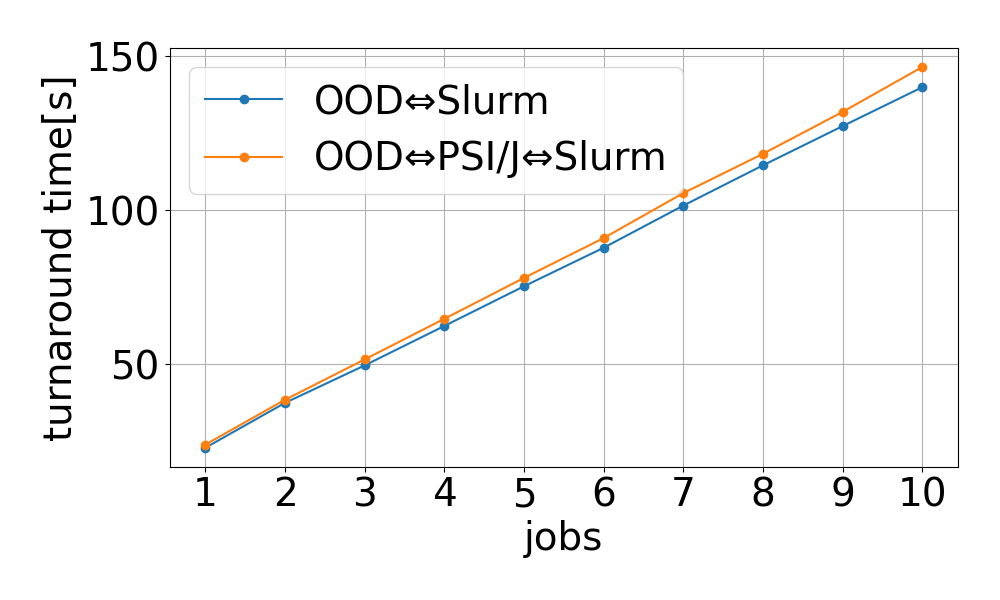
\includegraphics[width=100mm]{./fig/ave_1-20.png}
    \caption{機能分離前後でのターンアラウンドタイムの比較}
    \label{fig8}
\end{figure}
  
\begin{figure}[tb]
    \centering
    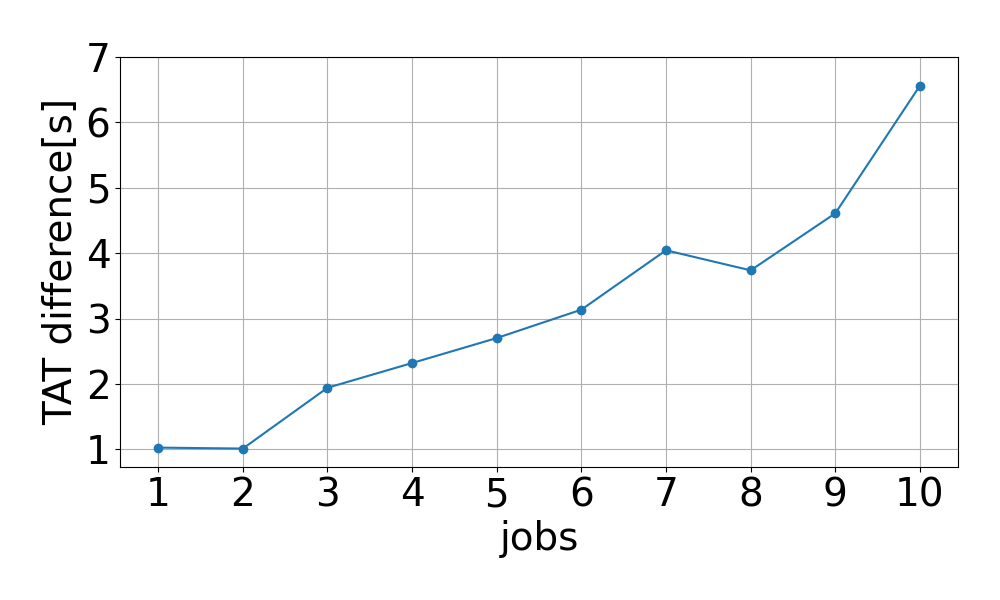
\includegraphics[width=100mm]{./fig/ave_diff_1-20.png}
    \caption{実行時オーバーヘッドの差}
    \label{fig9}
\end{figure}


ジョブを1~100回連続投入した際の機能分離前後でのターンアラウンドタイムの評価結果を図\ref{fig10}に示す.横軸は連続して投入したジョブの数,縦軸はターンアラウンドタイムを示す.1~10回の連続投入の場合と同じく,PSI/Jを経由した場合の方がわずかにターンアラウンドタイムが大きくなっており,連続投入するジョブ数を大きくしても極端にオーバヘッドに差が出ることはないということがわかった.\par
様々なジョブの連続投入回数でのターンアラウンドタイムの結果から,ジョブ実行時のオーバヘッドを測定した.その結果から,ジョブの連続投入回数に依らず,PSI/Jを経由した場合のオーバヘッドは,PSI/Jを経由しない場合のターンアラウンドタイムの5%以内に収まり,提案手法によって生じるオーバヘッドは十分無視できるといえる.\par

\begin{figure}[tb]
    \centering
    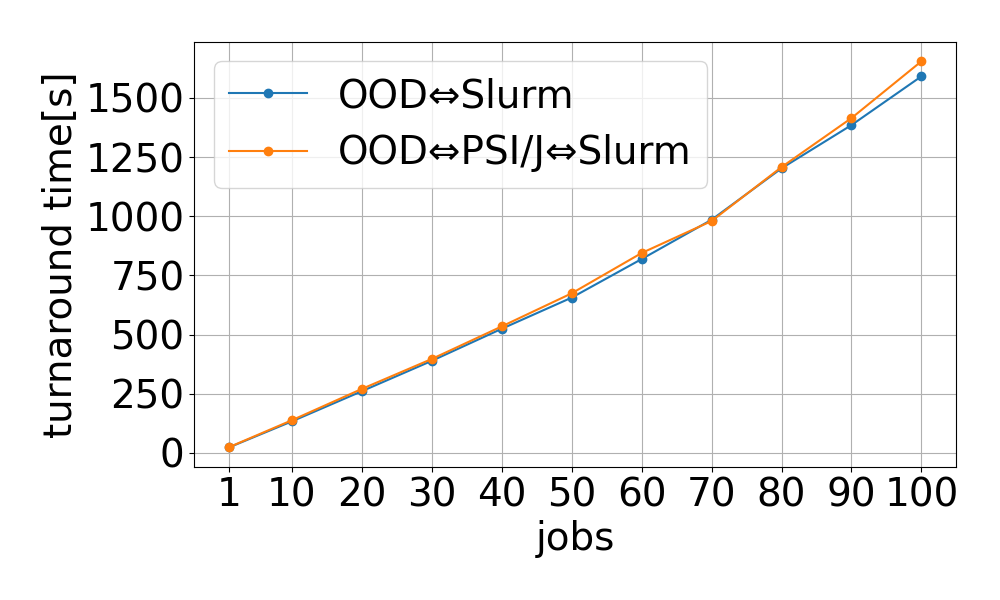
\includegraphics[width=100mm]{./fig/100jobs.png}
    \caption{ジョブ数を増加した際のターンアラウンドタイムの比較}
    \label{fig10}
\end{figure}

\subsection{結言}
本章では,実際にジョブの投入を行った際の提案手法の実装の評価結果を示した.はじめに,評価を行う環境について説明した.その後,機能の分離前後で生じるオーバヘッドを測定する際の評価条件について説明した.これらの評価環境と評価条件により得られた評価結果により,提案手法により生じるオーバヘッドは充分小さいため実用上は問題ないということを示した.\par